%You can leave alone everything before Line 79.
\documentclass{article}
\usepackage{url,amsfonts, amsmath, amssymb, amsthm,color, enumerate}
% Page layout
\setlength{\textheight}{8.75in}
\setlength{\columnsep}{2.0pc}
\setlength{\textwidth}{6.5in}
\setlength{\topmargin}{0in}
\setlength{\headheight}{0.0in}
\setlength{\headsep}{0.0in}
\setlength{\oddsidemargin}{0in}
\setlength{\evensidemargin}{0in}
\setlength{\parindent}{1pc}
\newcommand{\shortbar}{\begin{center}\rule{5ex}{0.1pt}\end{center}}
%\renewcommand{\baselinestretch}{1.1}
% Macros for course info
\newcommand{\courseNumber}{ME 552}
\newcommand{\courseTitle}{Mechatronics}
\newcommand{\semester}{Fall 2012}
\newcommand{\xxx}[1]{\textcolor{red}{#1}}
% Theorem-like structures are numbered within SECTION units
\theoremstyle{plain}
\newtheorem{theorem}{Theorem}[section]
\newtheorem{lemma}[theorem]{Lemma}
\newtheorem{corollary}[theorem]{Corollary}
\newtheorem{proposition}[theorem]{Proposition}
\newtheorem{statement}[theorem]{Statement}
\newtheorem{conjecture}[theorem]{Conjecture}
\newtheorem{fact}{Fact}
%definition style
\theoremstyle{definition}
\newtheorem{definition}[theorem]{Definition}
\newtheorem{example}{Example}
\newtheorem{problem}[theorem]{Problem}
\newtheorem{exercise}{Exercise}
\newtheorem{algorithm}{Algorithm}
%remark style
\theoremstyle{remark}
\newtheorem{remark}[theorem]{Remark}
\newtheorem{reduction}[theorem]{Reduction}
%\newtheorem{question}[theorem]{Question}
\newtheorem{question}{Question}
%\newtheorem{claim}[theorem]{Claim}
%
% Proof-making commands and environments
\newcommand{\beginproof}{\medskip\noindent{\bf Proof.~}}
\newcommand{\beginproofof}[1]{\medskip\noindent{\bf Proof of #1.~}}
\newcommand{\finishproof}{\hspace{0.2ex}\rule{1ex}{1ex}}
\def\therefore{\boldsymbol{\text{ }
\leavevmode
\lower0.4ex\hbox{$\cdot$}
\kern-.5em\raise0.7ex\hbox{$\cdot$}
\kern-0.55em\lower0.4ex\hbox{$\cdot$}
\thinspace\text{ }}}

\newenvironment{solution}[1]{\medskip\noindent{\bf Problem #1.~}}{\shortbar}

%====header======
\newcommand{\solutions}[4]{
%\renewcommand{\thetheorem}{{#2}.\arabic{theorem}}
\vspace{-2ex}
\begin{center}
{\small  \courseNumber, \courseTitle
\hfill {\Large \bf {#1} }\\
\semester, University of Michigan, Ann Arbor \hfill
{\em Date: #3}}\\
\vspace{-1ex}
\hrulefill\\
\vspace{4ex}
{\LARGE Lab Assignment #2}\\
\vspace{2ex}
\end{center}
\begin{trivlist}
\item \textsc{Team members:\\} {#4}
\end{trivlist}
\noindent
\shortbar
\vspace{3ex}
}
% math macros
\newcommand{\defeq}{\stackrel{\textrm{def}}{=}}
\newcommand{\Prob}{\textrm{Prob}}
%==
\usepackage{graphicx}
\usepackage{xfrac}
\begin{document}
%%%%%%%%%%%%%%%%%%%%%%%%%%%%%%%%%%%%%%%%%%%%%%%%%
%\solutions{Your name}{Problem Set Number}{Date of preparation}{Collaborators}{Prover}{Verifiers}
\solutions{}{2: MagLev}{\today}{Shiva Ghose, @gshiva\\ John Peterson, @jrpeters\\ Peter Turpel, @pturpel\\ Chan-Rong Lin, @pmelin}
%%%%%%%%%%%%%%%%%%%%%%%%%%%%%%%%%%%%%%%%%%%%%%%%%
%\renewcommand{\theproblem}{\arabic{problem}} 
%%%%%%%%%%%%%%%%%%%%%%%%%%%%%%%%%%%%%%%%%%%%%%%%%
%
% Begin the solution for each problem by
% \begin{solution}{Problem Number} and ends it with \end{solution}
%
% the solution for Problem 
\section*{Teamwork Participation Pledge :: Team 1}

I attest that I have made a fair and equitable contribution to this lab and submitted 
assignment. \\

My signature also indicates that I have followed the University of Michigan Honor Code, 
while working on this lab and assignment.\\

I accept my responsibility to look after all of the equipment assigned to me and my team, 
and that I have read and understood the X50 Lab Rules.\\

\begin{table}[h]
\begin{center}
    \begin{tabular}{|c|c|c|}
        \hline
        \textbf{Name} & \textbf{Email}     & \textbf{ \ \ \ \ \  \ \  \ \ \ \ \  \ \ Signature  \ \ \ \ \  \ \ \ \ \ \ \  \ \ } \\ \hline
        	~& ~& ~\\
	~& ~& ~\\
	Shiva Ghose   & gshiva@umich.edu   & ~                  \\
	~& ~& ~\\
	~& ~& ~\\ \hline 
	~& ~& ~\\
	~& ~& ~\\
        John Peterson & jrpeters@umich.edu & ~                  \\ 
	~& ~& ~\\
	~& ~& ~\\ \hline 
	~& ~& ~\\
	~& ~& ~\\
        Peter Turpel   & pturpel@umich.edu & ~                  \\
	~& ~& ~\\
	~& ~& ~\\ \hline 
	~& ~& ~\\
	~& ~& ~\\
        Chan-Rong Lin   & pmelin@umich.edu & ~                  \\
	~& ~& ~\\
	~& ~& ~\\ \hline 
        \hline
    \end{tabular}
\end{center}
\end{table}

\newpage

\section{Part 2 Question 1}

\subsection*{a.}

\subsubsection{Break Beam Sensor}

\textbf{Assumptions} \\
\begin{itemize}
\item Neglect Diffraction.
\item Light rays are parallel. 
\end{itemize}
As a consequence of these two assumptions the IR beam from the LED to the photo-transistor can be modeled as a cylinder.  The shadow casted by the sphere is then simply the circle with radius equal to the radius of the sphere.  This also means that the distance between the sphere and the IR LED does not matter, instead the only values that matter are the radius of the IR beam, the radius of the sphere, and the perpendicular distance between the axis of the beam and the center of the sphere.  The amount of light received by the photo-transistor can then simply be modeled as the intersection of two circles in 2-dimensions. \\

\[
  Radiance \hspace{0.1cm} Fraction = \left\{
  \begin{array}{l l}
    \frac{A_{beam} - A_{sphere}}{A_{beam}} & \quad \text{if } r_{sphere} + |d| < r_{beam} \\
    0 & \quad \text{if } r_{beam} + |d| < r_{sphere} \\
    1 & \quad \text{if } |d| < r_{beam} + r_{sphere} \\
    \frac{A_{beam} - A_{Overlap}}{A_{beam}} & \quad \text{if } |d| < r_{sphere} + r_{beam} \\
  \end{array} \right.
\]

\xxx{Format this part to look a bit nicer} \\
\textbf{Where:}
$$ A_{beam} = \pi r_{beam}^2 \hspace{1cm} A_{sphere} = \pi r_{sphere}^2 $$ 
$$ x = \frac{d^2+r_{beam}^2+r_{sphere}^2}{2d} \hspace{1cm} d_{beam}=x \hspace{1cm} d_{sphere}=d-x=\frac{d^2-r_{beam}^2+r_{sphere}^2}{2d} $$
$$ A_{Obeam} = r_{beam}^2 \cos^{-1} (\frac{d_{beam}}{r_{beam}})-d_{beam} \sqrt{r_{beam}^2-d_{beam}^2}$$ 
$$ A_{Osphere} = r_{sphere}^2 \cos^{-1} (\frac{d_{sphere}}{r_{sphere}})-d_{sphere} \sqrt{r_{sphere}^2-d_{sphere}^2}$$
$$ A_{Overlap} = A_{Obeam} + A_{Osphere} $$

\begin{figure}
\begin{center}
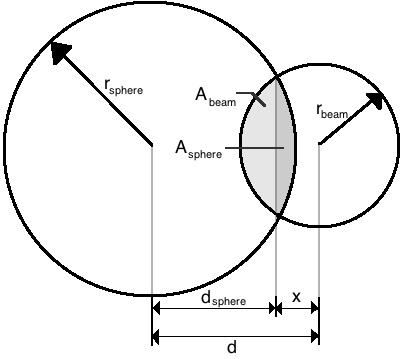
\includegraphics[width = 9cm]{beam_sphere_diagram.png}
\label{P2Q1_a1}
\caption{Planar approximation of IR beam occluded by steel sphere}
\end{center}
\end{figure}

\subsubsection{Electro Magnet}
\textbf{Assumptions}
\begin{itemize}
\item $ \mu_{Al} \approx \mu_{Cu} \approx \mu_{air} $ \\
\item $ \mu_{steel} \gg \mu_{air} $ \\
\item can model the steel sphere as a cylinder with its axis collinear with the electromagnet  \\ 
$$A_{cd} \approx A_{s} = \pi * r_{sphere}^2 $$ \\
\item neglect effects of fringing on cross-sectional area and assume particular dimensions of area of paths through the air that are consistent with the solid objects in the system \\
$$ A_{EM} = \pi*r_{EM}^2 \approx A_{ab} \hspace{1cm} A_{s} \approx A_{bc} \approx A_{de} \hspace{1cm} A_{EM} \approx A_{be} + A_{bc} $$ \\
\item Path length from b to c does not vary with x \\
$$ \frac{\partial}{\partial x} (L_{bc}) = 0$$ \\
\end{itemize}

Drawing out approximate flux paths yields the following diagram \xxx{make diagram of system} which can be converted to the following magnetic circuit shown in \xxx{magnetic circuit diagram} by applying Ampere's Law and Maxwell's $2^{nd}$ law which yield the following three equations.  \\

$$ NI = \phi \left (\mathbb{R}_{EM} + \mathbb{R}_{ab}\right) + \phi_{main} \left( \mathbb{R}_{bc}+\mathbb{R}_{s}+\mathbb{R}_{dc} \right) $$
$$ NI = \phi \left( \mathbb{R}_{EM} + \mathbb{R}_{ab} \right) + \phi_{leak} \left( \mathbb{R}_{be} \right) $$
$$ \phi = \phi_{main} + \phi_{leak} $$


$$ \mathbb{R}_{EM} = \frac{L_{EM}}{A_{EM}\mu_{air}}  \hspace{1cm} \mathbb{R}_{ab} = \frac{L_{ab}}{A_{EM}\mu_{air}} \hspace{1cm} \mathbb{R}_{bc} = \frac{L_{bc}}{(A_{s})\mu_{air}} \hspace{1cm} \mathbb{R}_{de} = \frac{x}{A_{A_{s}}\mu_{air}} \hspace{1cm} $$ $$ \mathbb{R}_{be} = \frac{L_{be}}{(A_{EM} - A_{s})\mu_{air}}  \hspace{1cm}  \mathbb{R}_{s} = \frac{2*r_{sphere}}{A_{s}\mu_{steel}} \approx 0$$

Solving the $2^{nd}$ equation for $\phi_{leak}$ gives:

$$\phi_{leak} = C_{0}\left( NI-C_{1}\phi_{main} \right)$$ 
$$C_{0} = \frac{\mu_{air} A_{EM} (A_{EM} - A_{s})}{L_{be} A_{EM} + (L_{EM} + L_{ab})(A_{EM} - A_{s}))} \hspace{1cm} 
C_{1} = \frac{L_{EM} + L_{ab}}{\mu_{air} A_{EM}} $$

Substituting back into the $1^{st}$ equation lets us solve for $\phi_{main}$ yielding: 

$$ \phi_{main} = \frac{NI(1-C_{0}C_{1})}{C_{1} - C_{0} C_{1}^2 + \frac{L_{bc}}{\mu_{air} A_{s}} + \frac{x}{\mu_{air} A_{s}}} $$

With equations for our fluxes we can now compute the self inductance and from that compute the force exerted on the steel sphere as a function of position and current.

$$ \lambda = N \phi = L(x) I $$
$$ W(i,x) = (\sfrac{1}{2}) L(x) I^2 = (\sfrac{1}{2}) N \phi(x) I =(\sfrac{1}{2}) N I (\phi_{main}(x) + \phi_{leak}(x))$$
$$ F(i,x) = \frac{d}{dx} (W(i,x) )= (\sfrac{1}{2}) N I ( \frac{d}{dx} (\phi_{main}) + \frac{d}{dx} (\phi_{leak})) $$

$$ \frac{d}{dx}(\phi_{main}) = - \frac{N I (1 - C_{0}C_{1} \mu_{air} A_{s}}{(\mu_{air} A_{s}(C_{1} - C_{0} C_{1}^2 + C_{2}) + x)^2} dx$$

$$ \frac{d}{dx}(\phi_{leak}) = -C_{0} C_{1} \frac{d}{dx}(\phi_{main})$$

Putting this pair of terms together yields our final expression for the force.

$$ F(x) = -\frac{1}{2} \left( 1 - C_{0}C_{1} \right)^2 \frac{\mu_{air} A_{s} N^2 }{(\mu_{air} A_{s}(C_{1} - C_{0} C_{1}^2 + C_{2}) + x)^2} I^2 $$

We can then condense these terms to arrive at a simple equation to model the force, shown below.  Where values for A and B can be obtained experimentally.

$$ F(x) = -\frac{A I^2}{(B+x)^2} $$

\subsubsection{Bearing \& Magnet System}

\subsection*{b.}

\subsection*{c.}

\subsection*{d.}

\subsection*{e.}

\subsection*{f.}

\subsection*{g.}

\section{Part 2 Question 2}

\subsection*{a.}

\subsection*{b.}

\subsection*{c.}

\subsection*{d.}

\section*{Question 3}

\end{document}